%\documentclass[conference]{IEEEtran}
\documentclass[10pt]{article}
%%%%%%%%%%%%%%%%%%%%%%%%%%%%%%%%%%%%%%%%%
% Lachaise Assignment
% Structure Specification File
% Version 1.0 (26/6/2018)
%
% This template originates from:
% http://www.LaTeXTemplates.com
%
% Authors:
% Marion Lachaise & François Févotte
% Vel (vel@LaTeXTemplates.com)
%
% License:
% CC BY-NC-SA 3.0 (http://creativecommons.org/licenses/by-nc-sa/3.0/)
% 
%%%%%%%%%%%%%%%%%%%%%%%%%%%%%%%%%%%%%%%%%

%----------------------------------------------------------------------------------------
%	PACKAGES AND OTHER DOCUMENT CONFIGURATIONS
%----------------------------------------------------------------------------------------

\usepackage{amsmath,amsfonts,stmaryrd,amssymb} % Math packages

\usepackage{enumerate} % Custom item numbers for enumerations
\usepackage{cite}
\usepackage[ruled]{algorithm2e} % Algorithms
\usepackage{indentfirst}
\usepackage[backref]{hyperref}
\usepackage[framemethod=tikz]{mdframed} % Allows defining custom boxed/framed environments

\usepackage{listings} % File listings, with syntax highlighting
\lstset{
	basicstyle=\ttfamily, % Typeset listings in monospace font
}

%----------------------------------------------------------------------------------------
%	DOCUMENT MARGINS
%----------------------------------------------------------------------------------------

\usepackage{geometry} % Required for adjusting page dimensions and margins

\geometry{
	paper=a4paper, % Paper size, change to letterpaper for US letter size
	top=2.5cm, % Top margin
	bottom=3cm, % Bottom margin
	left=2.5cm, % Left margin
	right=2.5cm, % Right margin
	headheight=14pt, % Header height
	footskip=1.5cm, % Space from the bottom margin to the baseline of the footer
	headsep=1.2cm, % Space from the top margin to the baseline of the header
	%showframe, % Uncomment to show how the type block is set on the page
}

%----------------------------------------------------------------------------------------
%	FONTS
%----------------------------------------------------------------------------------------
\usepackage[utf8]{inputenc} % Required for inputting international characters
\usepackage[T1]{fontenc} % Output font encoding for international characters

\usepackage{XCharter} % Use the XCharter fonts

%----------------------------------------------------------------------------------------
%	COMMAND LINE ENVIRONMENT
%----------------------------------------------------------------------------------------

% Usage:
% \begin{commandline}
%	\begin{verbatim}
%		$ ls
%		
%		Applications	Desktop	...
%	\end{verbatim}
% \end{commandline}

\mdfdefinestyle{commandline}{
	leftmargin=10pt,
	rightmargin=10pt,
	innerleftmargin=15pt,
	middlelinecolor=black!50!white,
	middlelinewidth=2pt,
	frametitlerule=false,
	backgroundcolor=black!5!white,
	frametitle={Command Line},
	frametitlefont={\normalfont\sffamily\color{white}\hspace{-1em}},
	frametitlebackgroundcolor=black!50!white,
	nobreak,
}

% Define a custom environment for command-line snapshots
\newenvironment{commandline}{
	\medskip
	\begin{mdframed}[style=commandline]
}{
	\end{mdframed}
	\medskip
}

%----------------------------------------------------------------------------------------
%	FILE CONTENTS ENVIRONMENT
%----------------------------------------------------------------------------------------

% Usage:
% \begin{file}[optional filename, defaults to "File"]
%	File contents, for example, with a listings environment
% \end{file}

\mdfdefinestyle{file}{
	innertopmargin=1.6\baselineskip,
	innerbottommargin=0.8\baselineskip,
	topline=false, bottomline=false,
	leftline=false, rightline=false,
	leftmargin=2cm,
	rightmargin=2cm,
	singleextra={%
		\draw[fill=black!10!white](P)++(0,-1.2em)rectangle(P-|O);
		\node[anchor=north west]
		at(P-|O){\ttfamily\mdfilename};
		%
		\def\l{3em}
		\draw(O-|P)++(-\l,0)--++(\l,\l)--(P)--(P-|O)--(O)--cycle;
		\draw(O-|P)++(-\l,0)--++(0,\l)--++(\l,0);
	},
	nobreak,
}

% Define a custom environment for file contents
\newenvironment{file}[1][File]{ % Set the default filename to "File"
	\medskip
	\newcommand{\mdfilename}{#1}
	\begin{mdframed}[style=file]
}{
	\end{mdframed}
	\medskip
}

%----------------------------------------------------------------------------------------
%	NUMBERED QUESTIONS ENVIRONMENT
%----------------------------------------------------------------------------------------

% Usage:
% \begin{question}[optional title]
%	Question contents
% \end{question}

\mdfdefinestyle{question}{
	innertopmargin=1.2\baselineskip,
	innerbottommargin=0.8\baselineskip,
	roundcorner=5pt,
	nobreak,
	singleextra={%
		\draw(P-|O)node[xshift=1em,anchor=west,fill=white,draw,rounded corners=5pt]{%
		Question \theQuestion\questionTitle};
	},
}

\newcounter{Question} % Stores the current question number that gets iterated with each new question

% Define a custom environment for numbered questions
\newenvironment{question}[1][\unskip]{
	\bigskip
	\stepcounter{Question}
	\newcommand{\questionTitle}{~#1}
	\begin{mdframed}[style=question]
}{
	\end{mdframed}
	\medskip
}

%----------------------------------------------------------------------------------------
%	WARNING TEXT ENVIRONMENT
%----------------------------------------------------------------------------------------

% Usage:
% \begin{warn}[optional title, defaults to "Warning:"]
%	Contents
% \end{warn}

\mdfdefinestyle{warning}{
	topline=false, bottomline=false,
	leftline=false, rightline=false,
	nobreak,
	singleextra={%
		\draw(P-|O)++(-0.5em,0)node(tmp1){};
		\draw(P-|O)++(0.5em,0)node(tmp2){};
		\fill[black,rotate around={45:(P-|O)}](tmp1)rectangle(tmp2);
		\node at(P-|O){\color{white}\scriptsize\bf !};
		\draw[very thick](P-|O)++(0,-1em)--(O);%--(O-|P);
	}
}

% Define a custom environment for warning text
\newenvironment{warn}[1][Warning:]{ % Set the default warning to "Warning:"
	\medskip
	\begin{mdframed}[style=warning]
		\noindent{\textbf{#1}}
}{
	\end{mdframed}
}

%----------------------------------------------------------------------------------------
%	INFORMATION ENVIRONMENT
%----------------------------------------------------------------------------------------

% Usage:
% \begin{info}[optional title, defaults to "Info:"]
% 	contents
% 	\end{info}

\mdfdefinestyle{info}{%
	topline=false, bottomline=false,
	leftline=false, rightline=false,
	nobreak,
	singleextra={%
		\fill[black](P-|O)circle[radius=0.4em];
		\node at(P-|O){\color{white}\scriptsize\bf i};
		\draw[very thick](P-|O)++(0,-0.8em)--(O);%--(O-|P);
	}
}

% Define a custom environment for information
\newenvironment{info}[1][Info:]{ % Set the default title to "Info:"
	\medskip
	\begin{mdframed}[style=info]
		\noindent{\textbf{#1}}
}{
	\end{mdframed}
}

\usepackage{url}
\usepackage{braket}
\usepackage{subcaption} % Include the file 
\usepackage{fancyhdr} %设置全文页眉、页脚的格式
\pagestyle{fancy}
\lhead{}           %页眉左边设为空
\chead{}           %页眉中间
\rhead{Peking University, EECS, Turing Class}           %页眉右边
%\rhead{\includegraphics[width=1.2cm]{1.eps}}  %页眉右侧放置lo
\lfoot{}          %页脚左边
\cfoot{\thepage}  %页脚中间
\rfoot{}          %页脚右边
 
 

 
 
 
 
 
 
\begin{document}

\title{\textbf{Quantum Networks: Architecture and Techniques}}

\author{Huiping Lin}

 \bibliographystyle{plain}
\maketitle
%\tableofcontents
\begin{abstract}
    In this paper, we will give a introduction on quantum networks, describing its architecture and usable techniques. We will follow the classical 5-layer network model, and give the quantum version of each layer, including related protocols and algorithms.
\end{abstract}

\section{Introduction}
With the development of quantum computing, information transitions between computing centers also become important. In classical computing world, we have computer networks, which link different computers and achieve communication between them. There have been plenty of theoretical and implementation research work on classical computer networks. Different network architecture model have been proposed, including the OSI model, and the TCP/IP model. In this paper, we will discuss the 5-layer TCP/IP model and extend this model to a quantum version.

The 5-layer TCP/IP model, including physical layer, link layer, network layer, transport layer and application layer, is an abstract model of real computer network. Different layers are responsible for different tasks using different protocols.

\section{Classical Network Architecture}

In classical computer world, networks help the computers use common communication protocols over digital interconnections to communicate with each other. Proper protocols are vital for achieving correct communications. By definition, a network protocol is an established set of rules that determine how data is transmitted between different devices in the same network. It's similar to human's communications. Speaking the same language simplifies communication between people, and some actions correspond to specific emotions (for example, smiling means friendly and shaking hands means cooperation). 

Network protocol stack model splits the communication process between two network devices into some layers. All the layers are self-contained, and the tasks assigned to them can be executed independently. And based on this model, network protocols divide the communication process into discrete tasks across every layer of the OSI model. One or more network protocols operate at each layer in the communication exchange.

Therefore, different level takes responsible for different tasks, and protocols occur at every level of networks.
% \section{}

Now we will introduce the 5-layer model, and each model's tasks and corresponding protocols.


\begin{itemize}
    \item Physical layer
    
    The physical layer provides an electrical, mechanical, and procedural interface to the transmission medium. The shapes and properties of the electrical connectors, the frequencies to broadcast on, the line code to use and similar low-level parameters, are specified by the physical layer.
    \item Link layer
    
    The data link layer, or layer 2, is the second layer of the seven-layer OSI model of computer networking. This layer is the protocol layer that transfers data between nodes on a network segment across the physical layer.[2] The data link layer provides the functional and procedural means to transfer data between network entities and may also provide the means to detect and possibly correct errors that can occur in the physical layer.

The data link layer is concerned with local delivery of frames between nodes on the same level of the network. Data-link frames, as these protocol data units are called, do not cross the boundaries of a local area network. Inter-network routing and global addressing are higher-layer functions, allowing data-link protocols to focus on local delivery, addressing, and media arbitration. In this way, the data link layer is analogous to a neighborhood traffic cop; it endeavors to arbitrate between parties contending for access to a medium, without concern for their ultimate destination. When devices attempt to use a medium simultaneously, frame collisions occur. Data-link protocols specify how devices detect and recover from such collisions, and may provide mechanisms to reduce or prevent them.


\item Network layer

The network layer provides the means of transferring variable-length network packets from a source to a destination host via one or more networks. Within the service layering semantics of the OSI network architecture, the network layer responds to service requests from the transport layer and issues service requests to the data link layer.

    \item Transport layer
    

    In computer networking, the transport layer is a conceptual division of methods in the layered architecture of protocols in the network stack in the Internet protocol suite and the OSI model. The protocols of this layer provide end-to-end communication services for applications.  It provides services such as connection-oriented communication, reliability, flow control, and multiplexing.

    \item Application layer
    
    The application layer contains the communications protocols and interface methods used in process-to-process communications across an Internet Protocol (IP) computer network.The application layer only standardizes communication and depends upon the underlying transport layer protocols to establish host-to-host data transfer channels and manage the data exchange in a client–server or peer-to-peer networking model. Though the TCP/IP application layer does not describe specific rules or data formats that applications must consider when communicating, the original specification (in RFC 1123) does rely on and recommend the robustness principle for application design.

\end{itemize}

\section{Quantum Network}

In this section, we will introduce some specific features of quantum network.

First, the transmisson of information is achieved by qubits, which is foundamentionally different from classical bits. The non-cloning theorem enables that qubits cannot be copied, which theoretically garantees the security of transmisson. Additionally, two qubits can share a special relation known as entanglement, even if these two qubits are stored at distant network nodes. This feature enables novel applications. 

However, the entanglement is short-lived, and can only be produced over short distances by sending photons over standard telecom fiber \cite{dynes2009efficient}. So how to enhance the entanglement and enable long-distance quantum communication is a vital problem.

\subsection{Physical Layer}

In classical networks, the physical layer is responsible for generating a stream of raw bits, and using physical medium for transmission, like microwave. Similarly, in quantum network, the physical layer enables the basic representation of information: qubits and entanglement between them. Therefore, the physical layer attempts entanglement generation. 

Physical layer should build entanglement between two devices, which lays groundwork for designing and implementing control and application protocols in platform independent software in order to build and scale quantum networks. There are already some quantum hardwares available to us, for example, NV platform which has achieved producing heralded entanglement using a solid state platform known as Nitrogen-Vacancy (NV) centres in diamond\cite{hensen2015loophole}. 
However, the same protocol could also be realized directly using Ion Traps\cite{moehring2007entanglement}
or Neutral Atoms\cite{hofmann2012heralded}.

The NV platform is an important platform realizing qubits transmission between two hosts. It is a few qubit quantum computer capable of arbitrary quantum gates, with an optical interface for initialization, measurement and entanglement generation. 

The NV center a point defect in the diamond lattice, and its most explored and useful property is its photoluminescence, which allows observers to read out its spin-state.
Additionally, NV centers in diamond have emerged as one of the most promising candidates for implementing quantum technologies because they exhibit long-lived spin quantum states and well-defined optical transitions\cite{childress2013diamond}. NV centers are typically produced from single substitutional nitrogen centers (called C or P1 centers in diamond literature) by irradiation followed by annealing at temperatures above 700 °C, and irradiation produces lattice vacancies, which are a part of NV centers. Those vacancies are immobile at room temperature. Key capabilities of the NV platform have already been demonstrated, including qubit lifetimes of 1.46 s, entanglement production faster than it is lost, and using entanglement to teleport qubits between separated NV centres. Other platforms' performance is not yet good enough to generate entanglement faster than it is lost.

Through all these advantages mentioned above, we can see that the NV platform is suitable for the realization of quantum networks. To use the NV platform to generate entanglement between two nodes $A$ and $B$ (capable of storing and manipulating qubits), an intermediate station called the heralding station $H$ should be connected to both $A$ and $B$ over optical fibers, which is responsible for entanglement swapping.

Each node can have two types of qubits: memory qubits as a local memory, and communication qubits with an optical interface. To produce entanglement, a time synchronized trigger is used at both $A$ and $B$ to create entanglement between each communication qubit, and a corresponding traveling qubit (photon). These photons are sent from $A$ and $B$ to $H$ over fiber. When both arrive at $H$, $H$ performs an automatic entanglement swapping operation which succeeds with some probability. Since $H$ has no quantum memory, both photons must arrive at $H$ at the same time to succeed.

In the case of success, one of several entangled states may be produced, which can however be converted to one other using local quantum gates at $A$ and $B$. After a generation attempt, the communication qubit may be moved to a memory qubit, in order to free the communication qubit to produce the next entangled pair. Many parameters influence the success and quality of this process, such as the quality of the qubits themselves, the probability of emission of a photon given a trigger signal, losses in fiber, and quality of the optical elements such as detectors used at $H$.

To teleport qubits between separated NV centres,
in \cite{dahlberg2019link}, an initial functional allocation of a quantum network stack is proposed, which illustrates the midpoint heralding protocol (MHP) at the physical layer. MHP is a lightweight protocol built directly on top of physical implementations of the form, supplementing them with some additional control information.
With minor modifications this MHP can be adapted to other forms of heralded entanglement generation between controllable nodes, even using multiple automated middle nodes.


The MHP protocol provides the two services, and takes the following actions.

\begin{itemize}
    \item  Protocol for Create and Keep (K)
    
    The parameters given to the MHP with a ``yes'' response contain the following:
    \begin{itemize}
        \item An ID for the attempt that is forwarded to $H$.
        \item Generation parameters $\alpha$(a microwave pulse prepares the communication
        qubit depending on the parameter $\alpha$).
        \item The device qubits for storing the entanglement.
        \item A sequence of operations to perform on the device memory.
    \end{itemize}
    The higher layer may instruct the MHP to perform a gate on the communication qubit depending on the heralding signal from $H$ allowing the conversion from the $\ket{\Psi^-}$ state to the $\ket{\Psi^+}$ state. Entanglement generation is then triggered at the start of the next time interval, including generation parameter $\alpha$, and a GEN message is sent to $H$ which includes a timestamp, and the given ID. The motivation for including the ID is to protect against errors in the classical control, for
    example losses.

    The station $H$ uses the timestamp to link the message to a detection window in which the accompanying photons arrived. Should messages from both nodes arrive, the midpoint verifies that the IDs transmitted with the GEN messages match, and checks the detection counts (Figure 3) from the corresponding detection window. The midpoint will then send a REPLY message indicating success or failure, and in the case of success which of the two states $\ket{\Psi^-}$ and $\ket{\Psi^+}$ were produced. The REPLY additionally contains a sequence number uniquely identifying the generated pair of entangled qubits chosen by $H$, which later enables the EGP to assign unique entanglement identifiers. This REPLY and the ID is forwarded to the link layer for post-processing. Note that the REPLY may be received many MHP cycles later, allowing the potential for emission multiplexing.
    \begin{figure}[htbp]
        \centering
        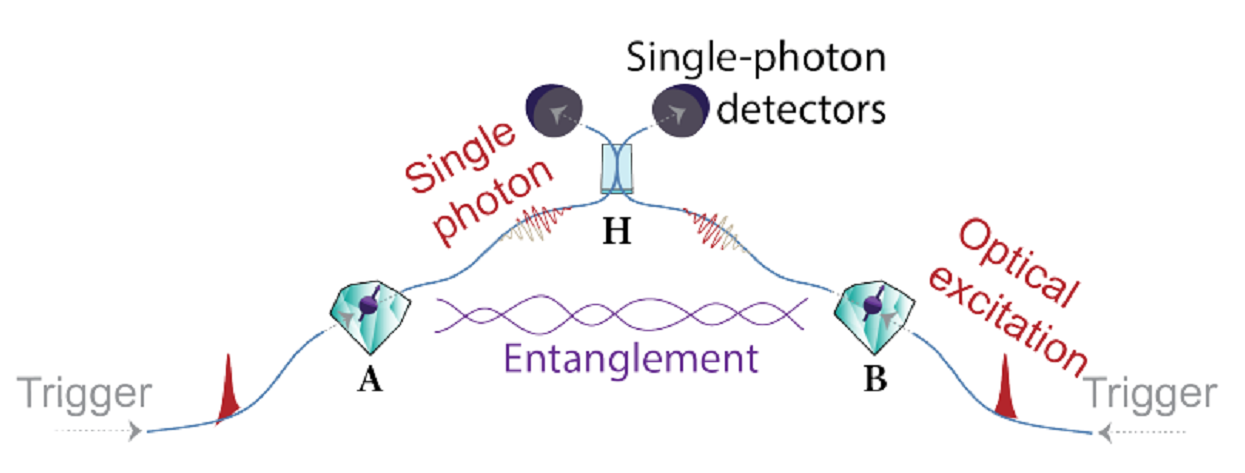
\includegraphics[width=0.45\textwidth]{figure/trigger.jpg}
        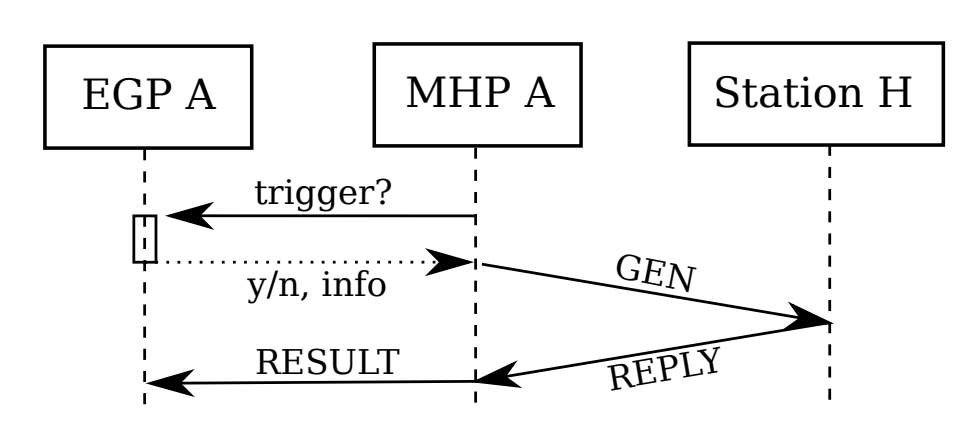
\includegraphics[width=0.45\textwidth]{figure/physical_layer.jpg}
        \caption{Entanglement Producer and Physical Layer Protocol.}
        \label{trigger}
    \end{figure}
    
    \item Protocol for Create and Measure (M)
    Handling M type requests is very similar, differing only in two ways:
    Instead of performing a gate on the communication qubit, the ``yes'' message requests the MHP to perform a measurement on the communication qubit in a specified basis once the photon has been emitted, even before receiving the response from $H$ . The outcome of the measurement and the REPLY are passed back to the EGP. In practice, the communication time from transmitting a GEN message to receiving a REPLY may currently exceed the duration of such a local measurement, and the MHP may choose to perform the measurement only after a successful response is received.



\end{itemize}


\subsection{Link Layer}

In classical networks, the link layer provides the functional and procedural means to transfer data between network entities. Additionally, it can detect and possibly correct errors that can occur in the physical layer. Therefore, the existence of the link layer helps make the transmission more reliable.


In quantum networks, entanglement has been already established in the physical layer, which means two devices are already connected to each other. The link layer is then to turn the physical layer making entanglement attempts into a robust entanglement generation service, that can produce entanglement between controllable quantum nodes connected by a (chain of) automated quantum nodes. So we have two tasks in general: 1) enhance the entanglement, and 2) do error correction.

Before describing further protocols, we introduce some exsiting techniques.

\subsubsection{Quantum Repeaters}

In \cite{briegel1998quantum}, quantum repeaters is proposed to help on this problem. As we've mentioned above, entanglement is short-lived, and prodused over short distances. The bottleneck for communication between distant nodes is the scaling of the error probability with the length of the channel connecting the nodes.  For channels such as an optical fiber, the probability for both absorption and depolarization of a photon (i.e., the qubit) grows exponentially with the length $l$ of the fiber. As a result, the number of trials scales exponentially with $l$ to transmit a photon without absorption, and when a photon arrives, the fidelity of the transmitted state decreases exponentially with $l$. Standard purification schemes\cite{bennett1996purification} can be used to solve the latter problem, but a certain minimum fidelity $F_{\min}$ is required, which cannot be achieved if $l$ is too large. Furthermore, in any realistic situation, the operations that are part of the purification protocol are themselves imperfect, and this defines a maximum attainable fidelity $F_{\max}$ and limits the efficiency of the scheme. 

Recall that in classical computer networks and classical communication, there are a type of devices called repeaters. Repeaters are used to extend transmissions so that the signal can cover longer distances or be received on the other side of an obstruction. The problem of exponential attenuation can be overcome by using repeaters at certain points in the channel, which amplify the signal and restore it to its original shape.

There are different types of repeaters, corresponding to different types of the signal's physical medium. For example, Figure \ref{repeater} shows the diagrammatic sketch and certain photo of radio repeaters.

\begin{figure}[htbp]
    \centering
    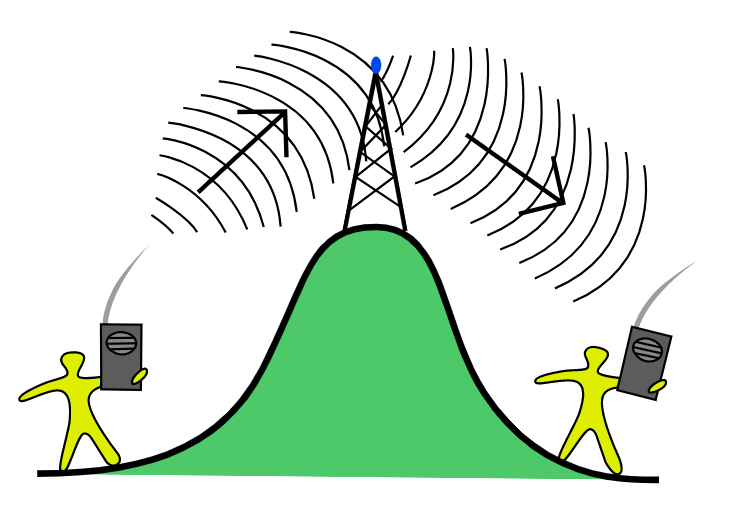
\includegraphics[width=0.4\textwidth]{figure/repeater.jpg}
    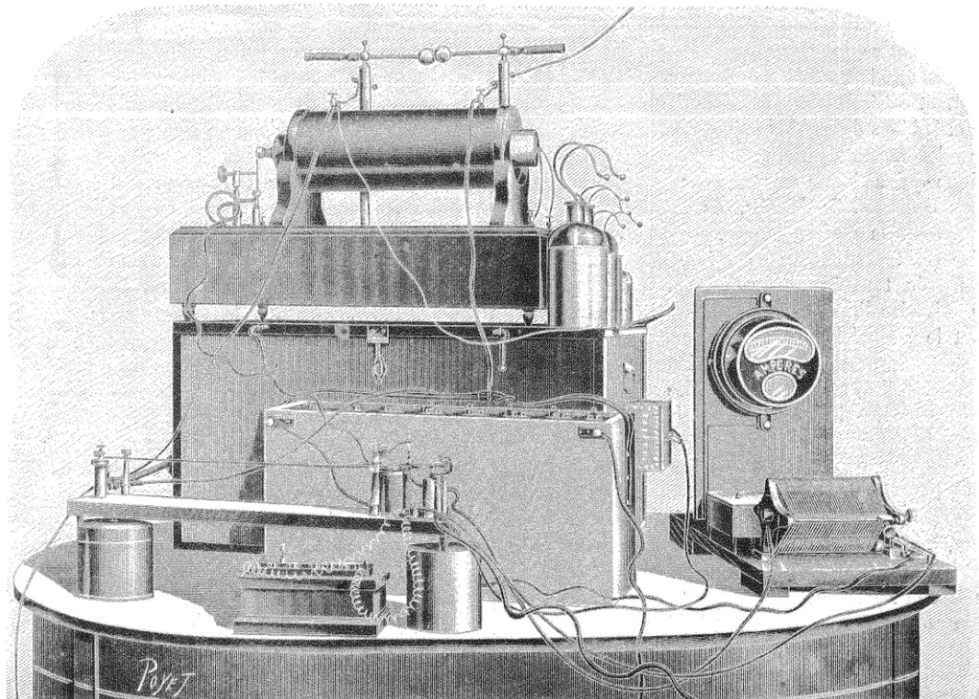
\includegraphics[width=0.4\textwidth]{figure/repeater2.jpg}
    \caption{Radio Repeaters.}
    \label{repeater}
\end{figure}

Guided by these ideas, for quantum communication between $A$ and $B$ over a long distance, we can divide the channel into $N$ segments with connection points in between. We then create $N$ elementary EPR pairs of fidelity $F_1$ between nodes $A$ and $C_1$, $C_1$ and $C_2$, ... , $C_n$ and $B$.  
Subsequently, we connect these pairs by making Bell measurements at the nodes $C_i$ and classically communicating the results between the nodes as in the schemes for teleportation\cite{vaidman1994teleportation} and entanglement swapping\cite{zukowski1993event}. This is totally similar to what we use in classical communication.

However, with every connection, the fidelity $F_0$ of the resulting pair may decrease: the connection process involves imperfect operations which introduce noise; and even for perfect connections, the fidelity decreases.
This may lead to an exponential decrease of the fidelity $F_N$ with $N$ of the final pair shared between $A$ and $B$. Eventually, the value of $F_N$ drops below $F_{\min}$, and therefore it will not be possible to increase the fidelity by purification. Therefore, the number of pairs $L$ that may be truly connected by this method seems therefore to be restricted by the condition $F_L<F_{\min}$.

Therefore, \cite{briegel1998quantum} proposed nested purification protocol, which combines
the methods of entanglement swapping and purification into a single (meta) protocol that circumvents this restriction. Its core idea is to use nested connection instead of sequential connection.
Assume that $N = L^n$ for some integer $n$. On the first level, we simultaneously connect the pairs (initial fidelity $F_1$) at all of the checkpoints except at $C_L,C_{2L},\cdots,C_{N-L}$. As a result, we have $N/L$ pairs of length $L$ and fidelity $F_L$ between $A$ and $C_L$, $C_L$ and $C_{2L}$, and so on. We also need to purify and obtain one pair of fidelity $\geq F_1$ on each segment by using $M$ copies that we construct in parallel fashion. Here $M$ depends on the initial fidelity, the degradation of the fidelity under connections, and the efficiency of the purification protocol. The total number of elementary pairs involved in constructing one of the more distant pairs of length $L$ is $LM$. 

On the second level, we connect $L$ of these more distant pairs at every checkpoint $C_{kL}(k = 1, 2, \cdots)$ except at $C_{L^2},C_{2L^2},\cdots,C_{N-L^2}$. As a result, we have $N/L^2$ pairs of length $L^2$, of fidelity $\geq F_L$. Again, we need $M$ parallel copies of these long pairs to repurify up to the fidelity $\geq F_1$. We iterate the procedure to higher and higher levels, until we reach the $n$th level. As a result, we have obtained a final pair between $A$ and $B$ of length $N$ and fidelity $\geq F_1$. In this way, the
total number $R$ of elementary pairs will be $(LM)^n$. Using this method, we are able to avoid the decrease of fidelity.


In general, the basic elements of the nested purification protocol are a) nested pair connections and b) purification. 

Quantum repeaters allow the creation of an entangled (EPR) pair of particles over arbitrary large distances with a tolerability of errors in the percent region. 

\subsubsection{Quantum Error Correction}
In the physical layer, we have introduced different error types on qubits, and a typical coding method Shor code, using 9 qubits to code a single-qubit. 

Actually, Shor code and many existing codes defined on qubits are examples of stabilizer codes. A detailed overview is presented in \cite{terhal2015quantum}, which reviews the theory of fault-tolerance and quantum error-correction, discuss
examples of various codes and code constructions. Stabilizer codes are attractive as (i) they are the straightforward quantum generalization of classical binary linear codes, (ii) their logical operators and distance are easily determined, and it is relatively simple to (iii) understand how to construct universal sets of logical gates and (iv) execute a numerical analysis of the code performance. The main idea of stabilizer codes is to encode $k$ logical qubits into n physical qubits using a subspace, the code space, $\mathcal L\subset (\mathbb{C}^2)^{\otimes n} $ spanned by states $\ket{\psi}$ that are
invariant under the action of a stabilizer group $\mathcal S$,
$$\mathcal{L}=\left\{|\psi\rangle \in\left(\mathbb{C}^{2}\right)^{\otimes n}: P|\psi\rangle=|\psi\rangle \quad \forall P \in \mathcal{S}\right\}.$$

Here $\mathcal S$ is an Abelian subgroup of the Pauli group, such that $-I\notin S$.

The physical layer may apply different encoding methods, and during the transmission, errors may occur at different stages. Then, we can use error-correction method to recover the qubits. Recall that in the physical layer is responsible for encoding, and the recovery after transmission happens in the link layer. Therefore, the physial layer and link layer together accomplish the quantum error correction task.

\subsection{Link Layer Protocol}
In this section, we will introduce some considerations on the design of link layer, and give a sketch of the link layer protocol according to \cite{dahlberg2019link}.

\subsubsection{Desired Service}

The link layer offers a robust entanglement creation service between a pair of controllable quantum nodes $A$ and $B$ that are connected by a quantum link. The process can be divided into two stages:

\begin{itemize}
    \item Requesting entanglement.
    
    Entanglement creation
    can be initiated at either $A$ or $B$ by a CREATE request from
    the higher layer with parameters. The parameters includes source node ID, purpose node ID, type of request, number of entangled pairs to be created, priority, the desired minimum
    fidelity and some other additional tags. 

    \item Response to entanglement requests.
    
    If entanglement has been produced successfully, an OK message should be returned. In addition, different use cases may desire several other pieces of information, which may also be tracked at higher layers. For example, if the request is CREATE, then the addtional information is a qubit ID for which identifies where the local qubit is in the quantum memory device; a priority value can also be set. In general, the link layer should response to the requests according to the instructions from higher layers.


    Evidently, these requests may suffer failures due to different reasons. There are many possibilities of failure resulting in the return of error messages. This includes:
    \begin{itemize}
        \item Timeout when a request could not be fulfilled in a specific time frame (TIMEOUT).
        \item An immediate rejection of the request because the requested fidelity is not achievable in the given time frame (UNSUPP).
        
        \item The quantum storage is too small to simultaneously store all pairs of an atomic request, permanently (MEMEXCEEDED) or temporarily (OUTOFMEM).
        
        \item Refusal by the remote node to participate (DENIED).
    \end{itemize}

    Finally, we allow an EXPIRE message to be sent, indicating that the entanglement is no longer available.

\item Fixed hardware parameters

There are parameters fixed for the specific hardware platform, or change only very infrequently. As such, these may be obtained by high-level software by querying the low level system periodically, similarly to some classical network architectures. These may include the number of available qubits, the qubit memory lifetimes and so on.

\end{itemize}


\subsubsection{Error Detection}

Proposals for enabling quantum communication by forward communication using quantum error correction also exist, which avoid entanglement swapping. However, these have arguably much more stringent requirements in terms of hardware, putting them in a technologically more distant future: they require the ability to create entangled states consisting of a large number of photons (only 10 realized today) and densely placed repeater stations performing near perfect operations.

We typically demand some minimum fidelity $F_{\min}$ with high confidence that may also fluctuate slightly for pairs produced within a time window.

we intersperse test rounds during entanglement generation to verify the quality of the link. Such test rounds are easy to produce without the need for complex gates or extra qubits. Evidently, there exists an exact analogy in the classical networking world, where we would transmit test bits to measure the current quality of transmission, e.g. a direct analogy to network profiling to gain confidence that the non-test bits are also likely to be transmitted with roughly the same amount of error. Yet, there we typically care about correctness of a specific data item, rather than an enabling resources like entanglement.

We now explain the test used to gain confidence in transmission quality, specifically to estimate the quality parameter fidelity $F$. The following is a standard procedure in quantum information to estimate the fidelity of a state $\rho$ to the entangled target state $\ket{\Psi^{-}}$. We emphasize that it is not possible to measure F from a single copy of the state $\rho$. The matrices $\rho$ are a mathematical description of an underlying quantum system, and not a matrix that one can read or access like classical information.

The fidelity $F$ measures how close a realized state $\rho$ is to an ideal target state $\ket{\Psi^{-}}$. The fidelity of a state ρ with the target
state can be written as

\begin{align}
F\left[\Psi^{-}\right]&=\left\langle\Psi^{-}|\rho| \Psi^{-}\right\rangle\\
&=1-\frac{\mathrm{QBER}_{X}+\mathrm{QBER}_{Y}+\mathrm{QBER}_{Z}}{2},
\end{align}
where for a fixed basis (say $Z$) the QBER (here ${\rm QBER}_Z$ ) is the probability of receiving equal measurement outcomes.

Let us first assume a simpler scenario, in which $n$ identical noisy entangled states $\rho$ are produced in succession and we want to estimate F . We remark that when using imperfect quantum devices it is evidently a highly idealized situation that all states $\rho$ are exactly identical. The testing protocol works as follows:

\begin{itemize}
    \item Node $A$ randomly chooses an $n$ element string $r = r_1,\cdots,r_n \in \{X,Z,Y \}$ and sends it to Node $B$.
    \item Nodes A and B now perform the following procedure for $n$ rounds: a) Node $A$ produces one entangled pair $\rho$ with Node $B$, b) Nodes $A$ and $B$ both measures their respective qubits in the basis $r_j$ and record outcomes $x_j^A$ (Node A) and $x_j^B$ (Node B) respectively.
    \item Node $B (A)$ transmits the outcome string $x_i^B(x_i^A)$ to Node $A (B)$.
    \item Both nodes estimate the error rates:
    \begin{align}
Q B E R_{Z} & \approx \frac{\#\left\{j \mid x_{j}^{A}=x_{j}^{B}, r_{j}=Z\right\}}{\#\left\{j \mid r_{j}=Z\right\}}, \\
Q B E R_{X} & \approx \frac{\#\left\{j \mid x_{j}^{A}=x_{j}^{B}, r_{j}=X\right\}}{\#\left\{j \mid r_{j}=X\right\}} \\
Q B E R_{Y} & \approx \frac{\#\left\{j \mid x_{j}^{A}=x_{j}^{B}, r_{j}=Y\right\}}{\#\left\{j \mid r_{j}=Y\right\}}
    \end{align}

\end{itemize}


\subsubsection{Link Layer Protocol}

For the link layer, \cite{dahlberg2019link} presents an implementation of link layer protocol called dubbed EGP, which is built up from different components:
\begin{itemize}
    \item Distributed Queue
    
    The EGP employs a distributed queue comprised of synchronized local queues at the controllable nodes. These local queues can be used to separate requests based on priority, where here we employ 3 for the different use cases (CK, NL, MD). We let one node hold the master copy of the queue, and use a simple two-way handshake for enqueing items, and
    a windowing mechanism to ensure fairness.

    \item Quantum Memory Management (QMM)
    
    The EGP uses the node’s quantum memory manager (QMM) to determine which physical qubits to use for generating or storing entanglement.


    \item  Fidelity Estimation Unit (FEU)
    
    In order to provide information about the quality of entanglement, the EGP employs a fidelit estimation unit. This unit is given a desired quality parameter $F_{\min}$, and returns generation parameters (such as $\alpha$) along with an estimated minimal completion time.
    Such a fidelity estimate can be calculated based on known hardware capabilities such as the quality of the memory and operations. To further improve this base estimate the EGP intersperses test rounds.

    \item Scheduler
    
    The EGP scheduler decides which request in the queue should be served next. In principle, any scheduling strategy is suitable as long as it is deterministic, ensuring that both nodes select the same request locally. This limits two-way communication, which adversely affects entanglement quality due to limited memory lifetimes.

    \item Protocol 
    
    Figure \ref{link protocol} presents an architecture diagram visualizing the operation. The protocol begins when a higher layer at a controllable node issues a CREATE operation to the EGP specifying a desired number of entangled pairs along with $F_{\min}$ and $t_{\max}$. Upon receipt of a request the EGP will query the FEU to obtain hardware parameters ($\alpha$), and a minimum completion time. 

    If this time is larger than $t_{\max}$, the EGP immediately rejects the request (UNSUPP). Should the request pass this evaluation, the local node will compute a fitting $min\_time$ specifying the earliest MHP polling cycle the request may begin processing. The node then adds the request into the distributed queue shared by the nodes. This request may be rejected by the peer should the remote node have queue rules that do not accept the specified purpose ID.
    Then, the EGP locally rejects the request (DENIED).

    \begin{figure}[htbp]
        \centering
        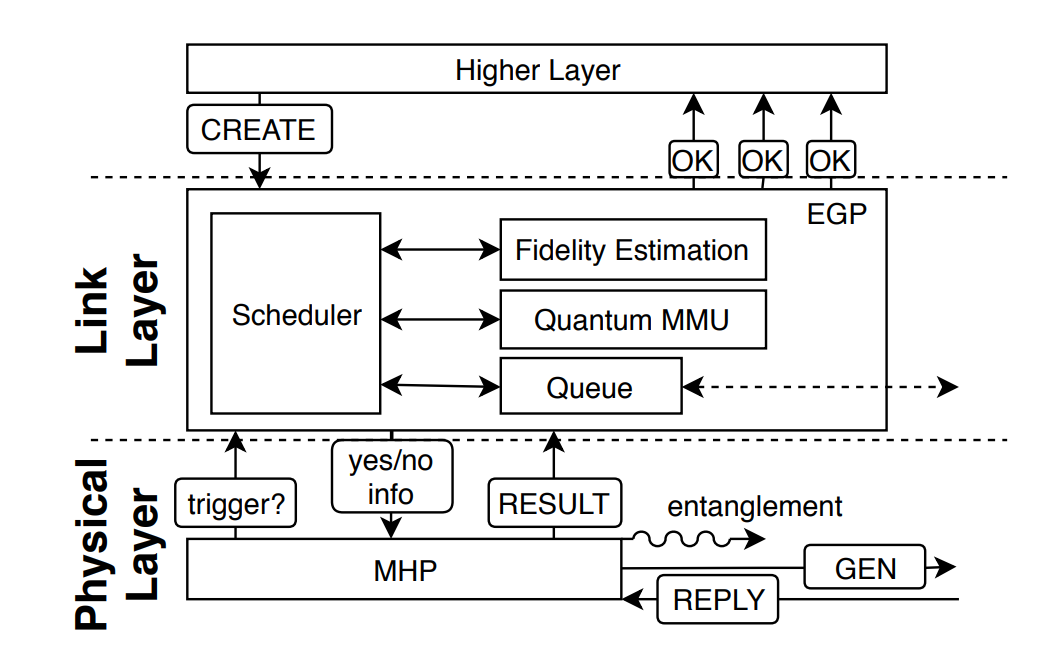
\includegraphics[width=0.6\textwidth]{figure/link_prorocol.jpg}
        \caption{Flow diagram of the MHP and EGP operation. The EGP handles CREATE requests and schedules entanglement generation attempts are issued to
        the MHP. Replies from the midpoint are parsed and
        forwarded to the EGP from request management.}
        \label{link protocol}
    \end{figure}

\end{itemize}

The local scheduler selects the next request to be processed, given that there exists a ready one (as indicated by $min\_time$). The QMM is then used to allocate qubits needed to fulfill the specified request type (create and keep $K$ or create and measure $M$). The EGP will then again ask the FEU to obtain a current parameter $\alpha$ due to possible fluctuations in hardware parameters during the time spent in the queue.
The scheduler then constructs a ``yes'' response to the MHP containing $\alpha$ from the FEU, along with an ID containing the unique queue ID of the request in the distributed queue, and number of pairs already produced for the request. This response is then forwarded to the local MHP upon its next poll to the EGP. If no request is ready for processing, a ``no'' response is returned to the MHP . At this point the MHP behaves as described in the previous section and an attempt at generating entanglement is made.
Whenever a REPLY and ID is received from the MHP, the EGP uses the ID to match the REPLY to an outstanding request, and evaluates the REPLY for correctness. Should the attempt be successful, the number of pairs remaining to be generated for the request is decremented and an OK message is propagated to higher layers.



In \cite{pant2019routing}, a single-link multipath routing (SLMP) algorithm is proposed and in \cite{chakraborty2019distributed} a virtual-path based greedy routing algorithm in ring and grid networks is proposed. The algorithms are both designed for entanglement routing in grid networks, and the latter one also contributes on formal restrictions of network layer considerations.


\subsection{Network Layer}

In the physical layer and link layer, we have described protocols that can make robust entanglement as well as error correction. Recall that in classical computing networks, the network layer is responsible for long-distance transmission of data, where routing is a vital problem.

\subsubsection{Network Topology}
For the network layer and higher layers, we do not seriously focus on how the entanglement is established physically, or the physical material of the links or channels. Instead, we abstract all the network components into a network topology, or a a multigraph $G = \langle V, E,C\rangle$. Here, $V$ is the set of $n$ nodes. Each node $u$ is a quantum processor or quantum repeater. A quantum processor is similar to an end host in classical networks, and is equipped with a limited number $Q_u$ of qubits. All quantum processors are connected via the classical Internet and are able to freely exchange classical information. And quantum repeaters are used to support long-distances entanglement sharing via quantum swapping. $E$ is the set of edges in the graph, and an edge existing between two nodes means that the two nodes share one or more quantum channels. A quantum channel connecting two nodes supports the transmission of qubits. The physical material of quantum channels may be polarization-maintaining optical fibers.
However, a quantum channel is inherently lossy: the success rate of each attempt to create an entanglement of a quantum channel $c$ is $p_c$ , which decreases exponentially with the physical length of the channel: $p_c = e ^{-\alpha L}$, where $L$ is the physical length of the channel and $\alpha$ is a constant depending on the physical media. If an attempt is successful, the two quantum processors share an entanglement pair, and there is a quantum link on this channel. The number of channels on an edge is called the width $W$ of the edge. $C$ is the set of all quantum channels, each of which is identified by its two end nodes. The number of channels on an edge is called the width $W$ of the edge.

There are also some restrictions on the abstract topology. A node can assign/bind each of its quantum memory qubits to a quantum channel, such that no qubit is assigned to more than one channel, and no channel is assigned more than one qubits at the same end of it. Channels that are assigned qubits at its both ends are bound channels, other channels are unbound channels. There could be more than one bound channels between two nodes. And two neighbor nodes may share multiple quantum links. To create a quantum entanglement, two neighbor nodes make a number of quantum entanglement attempts at the same time on the bound channels connecting them.



Similar to the classical network, in every attempt of connction, there must be a source node and a destination node. For convience, we will denote them as a S-D pair.

\subsubsection{Time Slots}

For multi-hop entanglement swapping, all nodes on the path need to establish and hold quantum entanglements with its predecessor and successor at the same time.  Hence, some level of time synchronization among all nodes is necessary, which can be achieved by existing current synchronization protocols via Internet connections. Time is loosely synchronized in time slots.
Each time slot is a device-technology-dependent constant and set to an appropriate duration such that the established entanglements do not discohere within one time slot. The global network topology $G = \langle V, E,C\rangle$, which is relatively stable, should be common knowledge for all nodes before any time slot.

The establishment of the connection can be viewed as $4$ phases in a time slot. Each phase has its own task:

\begin{figure}[htbp]
    \centering
    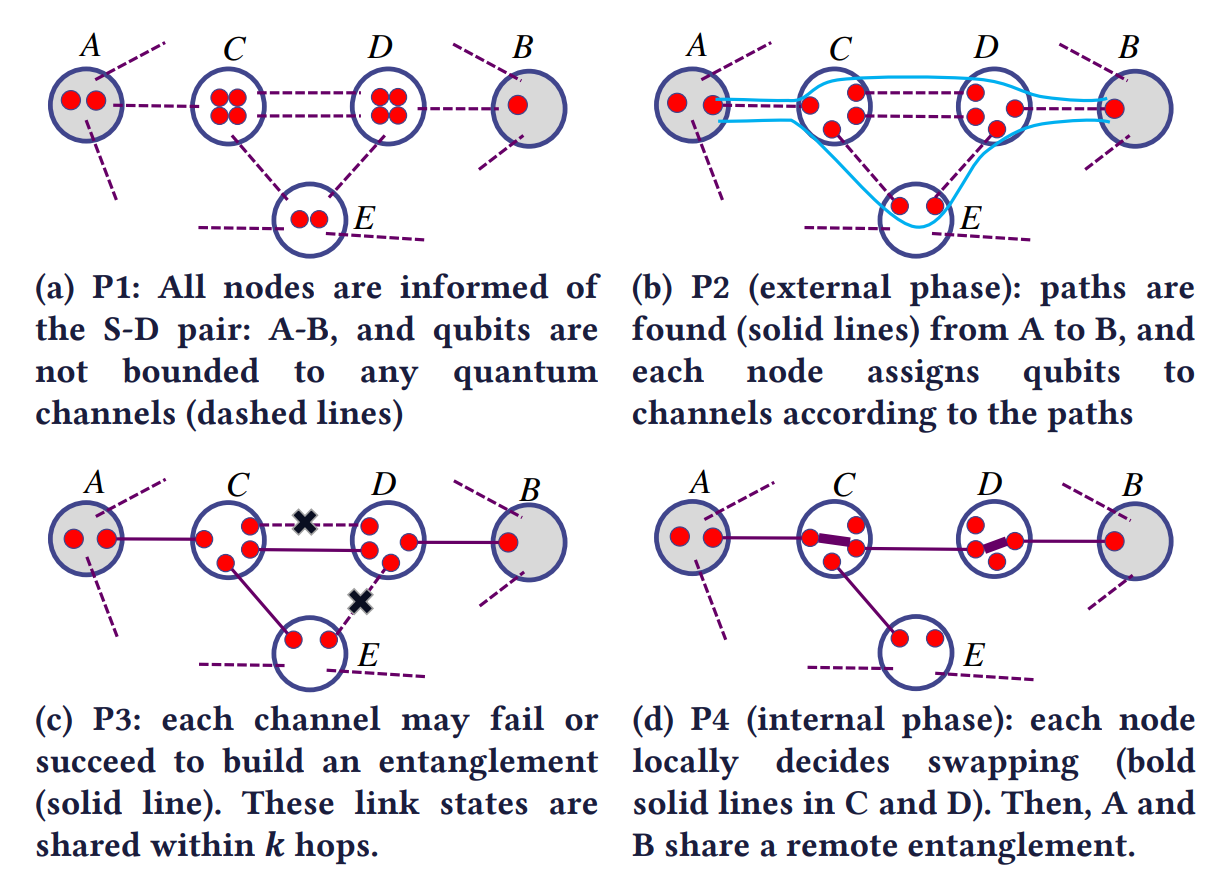
\includegraphics[width=0.7\textwidth]{figure/time_slot.jpg}
    \caption{Phases in a time slot.}
    \label{time slot}
\end{figure}


\begin{enumerate}
    \item Phase One (P1)
    
    All nodes receive the information of the current S-D pairs that need to establish long-distance entanglements. 

    \item Phase Two (P2)
    
    In Phase Two, also called the external phase, paths are found for the S-D pairs, according to an identical routing algorithm running on all nodes that produces consistency results. During P2, each channel can make a number $n_c\geq 1$ of attempts, until a link is built or timeout.
    After P2, some quantum links may be created.
    We call the information of these links as link states. Compared to
    the same term in link-state routing of classical networks, the
    quantum link states are highly dynamic and non-deterministic.
    
    \item Phase Three (P3)
    
    Each node knows its own link states via classical communications with its neighbors and shares its link states via the classical network. Since entanglements will quickly decay, each node can only exchange the link states with a subset of other nodes.

    \item Phase Four (P4)
    
    In Phase 4, also called the internal phase, nodes perform entanglement swapping to establish long-distance quantum entanglement using the successful quantum links. Each node locally determines the swapping of successful entanglements, which can be considered as placing an internal link between two qubits. Each swapping succeeds at a device-dependent probability $q$. A and B can successfully share an entanglement qubit pair (an ebit) if there is an end-to-end path with both external and internal links.
\end{enumerate}

After P4, the secret bit can be teleported from the source to the destination. Eavesdropping attempts at any repeater will be detected hence the confidentiality is preserved.

\subsubsection{Routing Problem}

We now give a formal definition of the entanglement routing problem.

Given a network topology $G = \langle V, E, C\rangle$, and a number of source-destination (S-D) pairs $\langle s_1, d_1\rangle, \langle s2,\\ d2\rangle,\cdots, \langle s_m, d_m\rangle$. The number of memory qubits of a node $u \in V$ is $Q_u$ , and each edge $e \in E$ consists of one or more channels from $C$. For each bound channel $c$, a link is successfully built at a probability $p_c$ in P2. In P3, each node gets the link-state information of its $k$-hop neighbors. Each node decides the swapping of its internal qubits in P4 locally, and each swapping succeeds in probability $q$. 

Our purpose of entanglement routing is to maximize the number of qbits delivered for all S-D pairs in each time slot, also the throughput in one time slot.

We can define a routing metric $E_t$, which indicates the expected expected throughput (EXT). For a $(W , h)$-path $P$ with $k$ hops and width $W$, suppose the success rate of a single channel on the $i$-th hop is $p_i$.  We denote the probability of the $k$-th hop on the path having exactly $i$ successful links as $Q_k^i$, and the probability of each of the first $k$ hops of $P$ has $\geq i$ successful links
as $P_k^i$. Then we get the recursive formula set, for $i\in\{1,2,\cdots,W\}$ and $k\in\{1,2,\cdots,h\}$:
\begin{align} 
    Q_{k}^{i} &=\left(\begin{array}{c}W \\ i\end{array}\right) p_{k}^{i}\left(1-p_{k}\right)^{W-i} \\
    P_{1}^{i} &=Q_{1}^{i} \\ 
    P_{k}^{i} &=P_{k-1}^{i} \cdot \sum_{l=i}^{W} Q_{k}^{l}+Q_{k}^{i} \cdot \sum_{l=i+1}^{W} P_{k-1}^{l} .
\end{align}

With each entanglement swapping successful probability $q$, the EXT is:
\begin{align}
    E_{t}=q^{h} \cdot \sum_{i=1}^{W} i \cdot P_{h}^{i},
\end{align}
and we want to maximize it.

\subsubsection{Routing Algorithms}

A single-link
multipath routing algorithm is proposed in \cite{pant2019routing}. It is a circuit-switching style protocol. It uses a greedy algorithm to choose the internal links: consider the subgraph induced by the successful external links and the repeater nodes (at the end of the external phase), and find in it the shortest path connecting Alice and Bob.
If no connected path between Alice and Bob exists, no shared ebits are generated in that time slot. If a shortest path of length $k_1$ is found, all internal links along the nodes of that path are attempted, and the probability a shared ebit is generated by this path is the probability that all $k_1−1$ internal link attempts were successful, i.e., $q^{k_1−1}$.
We then remove all the (external and internal) links of the above path from the subgraph, and find a shortest path connecting Alice and Bob in the pruned subgraph. Note that instead of removing the links of the first path from the subgraph, we could simply search for a shortest path in the original subgraph but one that is edge disjoint from the previous path. If such a path exists, we again attempt all internal links at the nodes of this path, so the probability the path contributes to the generation of an ebit between Alice and Bob is $q^{k_2−1}$, where $k_2$ is the length of the second path. And finally, the entanglement generation rate achieved using this greedy algorithm is the sum of expected rates from these paths.

In \cite{shi2020concurrent}, two concurrent routing algorithms are proposed: Q-PASS and Q-CAST.

The Q-PASS algorithm follows the four-phase time slot model with an additional offline phase. The core idea of Q-PASS is to pre-compute potential
``good'' paths between all possible S-D pairs based on the network topology $G$. 
The offline computation happens at the system initialization and
after the network topology change. Then in each time slot, every node uses an online algorithm to make qubit-to-channel assignments based on the precomputed paths of current S-D pairs and make local swapping decisions based on local link states. The design includes both offline and online algorithms.

However, the offline algorithm in Q-PASS has two fundamental disadvantages. 1) It has to compute candidate paths for $n(n-1)/2$ pairs because it does not know the runtime S-D pairs, where $n$ is the number of nodes. 2) The candidate paths exhibit a low utilization rate due to severe resource contention among them. As an opptimization, Q-CAST algorithm does not require any offline computation and always finds the paths if only paths exist in the residual graph.

Phase 1 and phase 3 only include standard processes
and do not have special algorithmic designs.  In phase 2, Q-CAST selects major paths for each S-D pair, without resource contention. Besides, contention-free recovery paths are also selected in phase 2. Phase 4 takes the major paths and recovery paths from Phase 2 and the link states from Phase 3 to compute the swapping decisions.

In phase 2, Q-CAST searches multiple contention-free paths for online S-D pairs using a greedy algorithm, which works as follows: Step 1) For every S-D pair, it uses the Extended Dijkstra’s algorithm to find the best path in terms of the routing metric EXT between this pair. Step 2) Among the best paths of all SD pairs, it further selects the path with the highest EXT and reserve the resources (qubits and channels) of this path, and the network topology is updated to the residual graph by removing the reserved resources. 
Steps 1) and 2) are repeated with the residual graph, until no more path can be found, or the number of paths exceeds a value limiting the number of paths to avoid unnecessary computation. 

Some extensions are also discussed to achieve better fairness and pioritized routing in \cite{shi2020concurrent}.

\subsection{Transport Layer Protocol}

In classical networks, the transport layer is usually responsible for providing reliable data transfer, and some additional services, such as congestion control. In classical networks, we have the TCP protocol, which provides reliable, ordered, and error-checked delivery of a stream of octets (bytes) between applications running on hosts communicating via an IP network.

In \cite{zhao2021redundant}, the first transport layer protocols are proposed for quantum networks, to be referred to as Quantum Transport Protocols (or QTPs). Additionally, in \cite{yu2021protocols}, a quantum version of TCP is proposed, which is called Quantum TCP. The QTPs are designed to handle the packet loss problem in transport, and further provide reliable, ordered, and error-checked delivery of a stream of octets (bytes) between applications running on quantum hosts communicating via an quantum network. 

We've mentioned the no-cloning theorem, which enables security during data transfer, but also prevents copying a qubit and re-transfer when encountering with packet loss. Therefore, the Q-TCP is proposed for dealing with packet loss problem uses quantum secret sharing techniques. As in detail, the Q-TCP use a quantum version three-way handshake protocol for connection establishment, and use secret sharin technique to enable retransmission protocol. 

The kernel of the retransmission protocol is a recursive use of the $(2,3)$ threshold scheme. The principle and technique of quantum secret sharing is proposed in \cite{cleve1999share}. The definition of $(m,n)$ threshold scheme can be generally explained as: use $n$ qubits to encode $1$ qubit, and only taking $\geq m$ qubits enables the recovery of the original qubit. This protocol chooses the $(2,3)$ threshold scheme for illustration of quantum retransmission, and the $(2,3)$ threshold scheme is qutrit-based (a three level quantum system); we can simply represent a qutrit by two qubits without using the fourth level. 

The protocol works as follows:
\begin{itemize}
    \item A quantum message $A$ is encoded into three shares $A_1A_2A_3$ and at least two shares are required to recover the message.
    \item The shares $A_2$ and $A_3$ are sent sequentially, depending on the acknowledgment of the previous share. If the first share $A_2$ is acknowledged, the share $A_3$ is directly sent. If $A_3$ is also acknowledged, we are done since $A_2A_3$ is enough for recovering $A$. 
    \item If $A_2$ gets lost, $A_1$ has to be sent carefully. So $A_1$ is then encoded into three shares by the $(2,3)$ threshold scheme and the procedure proceeds recursively.
\end{itemize}

A pseudocode is shown in Fig.\ref{retransmission}.

\begin{figure}[htbp]
    \centering
    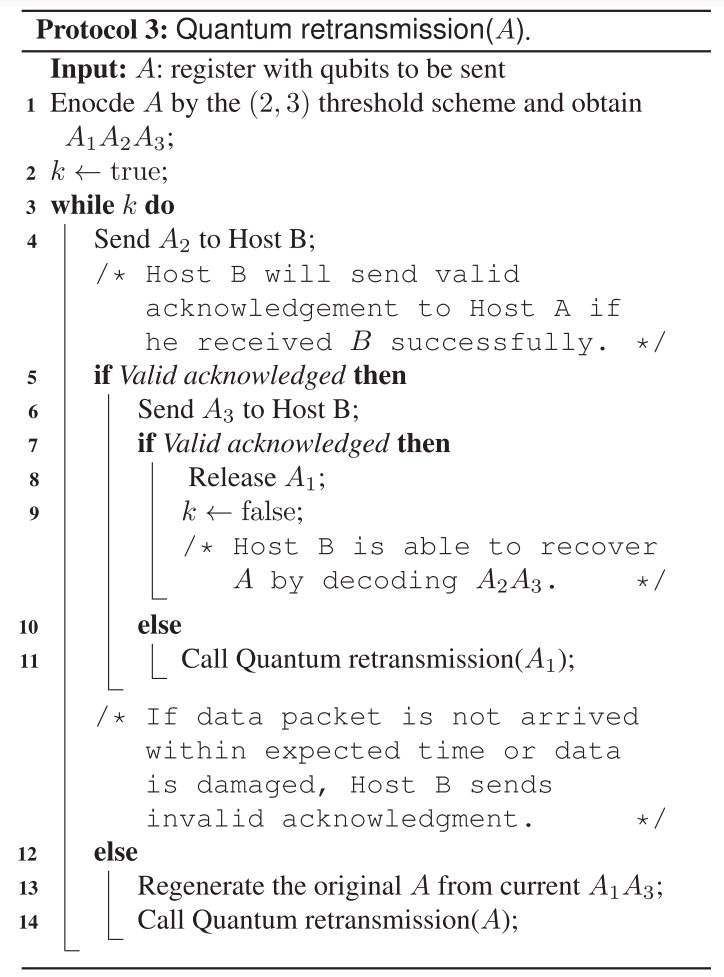
\includegraphics[width=0.4\textwidth]{figure/algo.jpg}
    \caption{Quantum retransmission protocol.}
    \label{retransmission}
\end{figure}


Based on the retransmission protocol and teleportation protocol, \cite{zhao2021quantum} proposes a transport layer protocol Tele-QTP, which takes the AIMD algorithm as the underlying algorithm. 

In a Teleportation QDN(Tele-QDN), two parties use the teleportation protocol for exchanging quantum information. Alice needs to first establish $W$ entanglement circuits in a time slot with Bob, if Alice wants to teleport $W$ qubits (because only one qubit can be teleported per circuit). This means Alice and Bob each needs to use at least $W$ qubits of quantum memory, and at least $2W$ qubits of quantum memory at each of the intermediate repeaters.
Unlike in a classical network, where congestion may occur during the actual data transmissions of TCP segments for example, here, the main challenge becomes how to establish these circuits given the limited quantum memory at each repeater, since once these circuits are established, teleportation of actual data qubits will not experience any congestion.

In a typical implementation of a distributed reservation approach, each source sends a request (in the classical network) for $W$ circuits along a path to the corresponding destination (Bob), where the path is determined by a quantum routing protocol. Such a distributed protocol typically has two phases: a forward phase and a backward phase. In the forward phase, each request is processed hop-by-hop by local controllers co-located with the quantum repeaters to see if $W$ entanglement links can be established and then forwarded to the next hop (controller) for further processing until it reaches the destination. At this time, the forward phase ends and the backward phase will start.

Recall that in a AIMD based TCP congestion control mechanism, the basic idea is to allow each source to request say $W$ circuits in one
time slot and $W+1$ circuits in the next if possible. If/when there isn't a sufficient amount of quantum memory at a given hop to satisfy all the requests from different sources, the protocol will cut the number circuits granted to a given source by half. In order to facilitate the presentation, hereafter, we use the terms common in TCP congestion control such as "sending window size" and "congestion encountered", respectively to refer to the number of circuits to be established, and to indicate whether the total number of requested circuits through a given repeater has exceeded the number of quantum memory it has or not. Note that other heuristics can also be used, and we leave them for future studies.


During the first step (i.e., the forward phase), Alice announces the desired sending window size, $W$, (or equivalently a request to reserve $W$ circuits) along a pre-selected path by routing protocols. After receiving this announcement (or request), every repeater along the path takes note of the requested window size, and waits for similar announcements from other QTP sessions to arrive.
Note that every source who wants to establish entanglement circuits in this time slot must either send out their announcements at the start of the time slot (or at the beginning of the
next time slot). Assuming that it takes at most $W$ units of time for an announcement from Alice to reach Bob, then no other destination can start Step Two earlier (even though it has already received all the announcements from other ingress nodes).

In Step Two (the backward phase), Bob initializes a response message and sends it back to Alice (along the same path but in reverse direction). The response message contains a Congestion Experienced (CE) flag to indicate if there is congestion along the selected path. The sending window size will be cut to if and only if the CE flag is set by any node.

More specifically, when a node receives (or Bob initializes) a response message, it will first check if the CE flag has been set already or not. If so, it forwards the response message to its upstream node, and tries to set up $W/2$ entanglement links with its upstream node (towards Alice). If the CE flag is not yet set, the node will determine if it can accommodate all circuits requested by all sources that will go through this node. In other words, for each and every QTP session requesting $W$ circuits going through this node, it will determine if it could allocate a total of $2W$ units of quantum memory for the QTP session. If it could, it will establish $W$ entanglement links with its downstream quantum node (towards Bob) and forwards the response message without setting the CE flag. Otherwise, this QTP session’s sending window size will be cut to half (as to be explained, Tele-QTP has built-in mechanisms to ensure that all nodes along the path can handle at least $W/2$ entanglement links per hop for this QTP session during this time slot. Accordingly, none of the other upstream repeater nodes will need to cut the sending window size any further. More specifically, this repeater node will do the following: (i). set the CE flag, and send the response to an upstream node; (ii). allocate $W/2$ units of quantum memory for each direction (upstream and downstream); and (iii). establish $W/2$ entanglement links with both its upstream and downstream nodes. In any case, once an entanglement link with its upstream node has been established, the repeater will perform a BSM operation and send the BSM result to Bob. Such an operation can take place while other upstream repeaters process the response message. Meanwhile, Bob will store the BSM result, along with the BSM results from all other repeater along the path, and use them when Alice performs a teleportation and sends her BSM results to Bob.

\bibliography{ref}

\end{document}
